\documentclass[12pt,a4paper]{report}

% ---------------------------------------------------------------------------
% PACKAGES
% ---------------------------------------------------------------------------
\usepackage[a4paper,left=1.2in,right=1in,top=1in,bottom=1in]{geometry}
\usepackage{mathptmx}              % Times-like font
\usepackage[T1]{fontenc}
\usepackage[english]{babel}
\usepackage{setspace}
\usepackage{titlesec}
\usepackage{tocloft}
\usepackage{fancyhdr}
\usepackage{graphicx}
\usepackage{tikz}
\usetikzlibrary{positioning, arrows.meta, shapes.geometric, fit}
\usepackage{booktabs}
\usepackage{array}
\usepackage{longtable}
\usepackage{caption}
\usepackage{enumitem}
\usepackage{listings}
\usepackage[hidelinks]{hyperref}
\usepackage{xcolor} % used only to define pure black/gray, no bright colors
\usepackage{amsmath}
\usepackage{graphicx}
% ---------------------------------------------------------------------------
% EDIT THESE BEFORE SUBMITTING — everything else in the report is generated
% from these seven lines.
% ---------------------------------------------------------------------------
\newcommand{\universityname}{Sylhet Engineering College}
\newcommand{\departmentname}{Department of Computer Science and Engineering}
\newcommand{\coursetitle}{Software Development III}
\newcommand{\coursecode}{CSE 600}
\newcommand{\studentname}{MD. Nayme Ur Rabiul Ruhan}
\newcommand{\studentid}{2021331514}
\newcommand{\supervisorname}{MD. Abu Naser Majumder}
\newcommand{\supervisordesig}{Associate Professor ,\\ \departmentname}
\newcommand{\submissiondate}{July 27, 2026}

% ---------------------------------------------------------------------------
% COLOR — grayscale only, on purpose. No accent colors anywhere in the report.
% ---------------------------------------------------------------------------
\definecolor{inkblack}{RGB}{20,20,20}
\definecolor{ruleline}{RGB}{120,120,120}
\definecolor{lightgray}{RGB}{235,235,235}

% ---------------------------------------------------------------------------
% Chapter / section heading style — plain, bold, no color, no boxes.
% ---------------------------------------------------------------------------
\titleformat{\chapter}[block]
  {\bfseries\Large}
  {\thechapter.}
  {0.5em}
  {\Large}
\titlespacing*{\chapter}{0pt}{0pt}{20pt}

\titleformat{\section}{\bfseries\large}{\thesection}{0.6em}{}
\titleformat{\subsection}{\bfseries\normalsize}{\thesubsection}{0.6em}{}

% ---------------------------------------------------------------------------
% Header / footer — simple, no rules of color
% ---------------------------------------------------------------------------
\pagestyle{fancy}
\fancyhf{}
\renewcommand{\headrulewidth}{0.4pt}
\fancyhead[L]{\small\leftmark}
\fancyhead[R]{\small\rightmark}
\fancyfoot[C]{\thepage}
\renewcommand{\chaptermark}[1]{\markboth{\thechapter.\ #1}{}}
\renewcommand{\sectionmark}[1]{\markright{\thesection\ #1}}

% ---------------------------------------------------------------------------
% Code listings — deliberately monochrome (bold/italic for emphasis, no color)
% ---------------------------------------------------------------------------
\lstset{
  basicstyle=\ttfamily\footnotesize,
  keywordstyle=\bfseries,
  commentstyle=\itshape,
  stringstyle=\ttfamily,
  showstringspaces=false,
  breaklines=true,
  breakatwhitespace=false,
  frame=single,
  framerule=0.4pt,
  numbers=left,
  numberstyle=\tiny,
  numbersep=8pt,
  tabsize=2,
  captionpos=b,
  xleftmargin=1.2em,
}


\lstdefinelanguage{JavaScript}{
  keywords={break,case,catch,const,continue,debugger,default,delete,do,else,
    export,false,finally,for,function,if,import,in,instanceof,let,new,null,
    return,switch,this,throw,true,try,typeof,var,void,while,with},
  sensitive=true,
  comment=[l]{//},
  morecomment=[s]{/*}{*/},
  morestring=[b]",
  morestring=[b]',
}

\captionsetup{font=small, labelfont=bf}

\setstretch{1.35}

\title{PDFly: A Web-Based PDF Utility Suite}
\author{\studentname}
\date{\submissiondate}

% ===========================================================================
\begin{document}
% ---------------------------------------------------------------------------
% TITLE PAGE
% ---------------------------------------------------------------------------
\begin{titlepage}
\centering

\vspace*{0.5cm}

% Logo (without figure environment)

\includegraphics[width=0.3\textwidth]{logo}

\vspace{0.4cm}

{\Large \universityname\par}
\vspace{0.15cm}
{\large \departmentname\par}

\vspace{0.8cm}

\rule{0.85\textwidth}{0.6pt}

\vspace{0.45cm}

{\Huge\bfseries PDFly\par}

\vspace{0.25cm}

{\Large A Web-Based PDF Utility Suite\par}

\vspace{0.45cm}

\rule{0.85\textwidth}{0.6pt}

\vspace{1cm}

{\Large\bfseries \coursetitle\ (\coursecode)\par}

\vspace{1.4cm}

\noindent
\begin{minipage}[t]{0.47\textwidth}
\centering
\textbf{Submitted by}\\[6pt]
\studentname\\
ID: \studentid
\end{minipage}
\hfill
\begin{minipage}[t]{0.47\textwidth}
\centering
\textbf{Submitted to}\\[6pt]
\supervisorname\\
\supervisordesig
\end{minipage}

\vfill

{\large \submissiondate\par}

\end{titlepage}

% ---------------------------------------------------------------------------
% FRONT MATTER
% ---------------------------------------------------------------------------
\pagenumbering{roman}



\chapter*{Acknowledgement}
\addcontentsline{toc}{chapter}{Acknowledgement}
I would like to express my sincere gratitude to \supervisorname\ for the guidance, feedback, and
supervision provided throughout the duration of this project. I am also thankful to the
\departmentname\ at \universityname\ for providing the resources and the opportunity to undertake
a practical, full-stack software project as part of this course. Finally, I acknowledge the
open-source communities behind Flask, React, and the various PDF-processing libraries used in
this project, whose documentation and tools made this work possible.

\chapter*{Abstract}
\addcontentsline{toc}{chapter}{Abstract}
Portable Document Format (PDF) files are the de facto standard for sharing documents that must
look the same on every device, but everyday tasks such as merging, splitting, compressing, or
converting them usually require either a desktop application or a third-party web service that
the user's files must be uploaded to and trusted with. This project, \textbf{PDFly}, is a
self-contained, full-stack web application that performs ten common PDF operations --- merge,
split, rotate, page-level editing, PDF-to-image conversion, image-to-PDF conversion, PDF-to-Word
conversion, Word-to-PDF conversion, compression, and watermarking --- entirely on a server that
the developer controls, with every uploaded and generated file deleted immediately after the
response is sent. The system consists of a Flask REST API backend that wraps a set of
well-established PDF-processing libraries and command-line tools (pypdf, ReportLab, Poppler,
Ghostscript, LibreOffice, and Tesseract OCR), and a React single-page frontend that presents the
ten tools as a categorized, card-based home page and a two-pane tool page, styled after
commercial PDF utility suites but on a dark, distraction-free canvas. The report documents the
requirement analysis, system architecture, implementation details of each module, the manual and
functional testing performed against the live server, and the issues encountered and resolved
during development, and concludes with a discussion of the system's limitations and directions
for future work.
\newpage
\tableofcontents
\listoffigures
\listoftables

\chapter*{List of Abbreviations}
\addcontentsline{toc}{chapter}{List of Abbreviations}
\begin{table}[h]
\centering
\begin{tabular}{@{}ll@{}}
\toprule
\textbf{Abbreviation} & \textbf{Full Form} \\
\midrule
API & Application Programming Interface \\
CORS & Cross-Origin Resource Sharing \\
CSS & Cascading Style Sheets \\
FR & Functional Requirement \\
HTTP & Hypertext Transfer Protocol \\
JSON & JavaScript Object Notation \\
OCR & Optical Character Recognition \\
PDF & Portable Document Format \\
REST & Representational State Transfer \\
SPA & Single Page Application \\
SRS & Software Requirements Specification \\
UI & User Interface \\
UUID & Universally Unique Identifier \\
WSGI & Web Server Gateway Interface \\
\bottomrule
\end{tabular}
\end{table}

% ---------------------------------------------------------------------------
% MAIN MATTER
% ---------------------------------------------------------------------------
\clearpage
\pagenumbering{arabic}

% =========================================================================
\chapter{Introduction}
% =========================================================================

\section{Background}
The Portable Document Format has become the standard container for documents that must be
shared while preserving exact layout and formatting. In practice, however, the file people
receive is rarely in the exact shape they need it: a scanned form may need to be rotated, two
separate reports may need to be merged into one, a document may need to be compressed before it
can be emailed, or a contract in PDF form may need to be edited in Word. Free web services such
as iLovePDF and SmallPDF solve this problem, but they require uploading potentially sensitive
documents to a third party, and most bundle these tools behind advertising, account walls, or
daily usage limits.

\section{Problem Statement}
There is a need for a lightweight, self-hosted alternative that performs the same set of common
PDF operations without any of the above trade-offs: no third-party storage, no account, no
artificial limits, and no advertising, while remaining simple enough to be understood, built, and
maintained by a single developer as a semester project.

\section{Objectives}
The project was carried out with the following objectives:
\begin{enumerate}[label=\arabic*.]
  \item To design and implement a REST API backend that exposes a distinct endpoint for each of
        the ten PDF operations listed in the abstract.
  \item To ensure that no uploaded or generated file persists on the server beyond the lifetime
        of a single request, using both an immediate post-request cleanup hook and an
        independent background sweep as a safety net.
  \item To validate every upload (file type, MIME type, size, and filename) before it reaches any
        processing logic, and to return clear, consistent error messages on failure.
  \item To build a single-page React frontend that presents every tool on one home page and
        allows the user to switch between tools without re-navigating to the home page.
  \item To verify the system end-to-end against a running server rather than relying only on a
        successful build.
\end{enumerate}

\section{Scope}
The system is scoped to single-user, stateless PDF processing. It does not include user accounts,
persistent storage, a database, or collaborative features. All processing is synchronous:
a request is answered with either the processed file or a JSON error object.

\section{Report Organization}
Chapter 2 reviews existing tools and positions this project relative to them. Chapter 3 presents
the requirement analysis and system design. Chapter 4 describes the implementation of the
backend and frontend in detail. Chapter 5 documents the testing performed, including two defects
found and fixed during a later verification pass. Chapter 6 discusses the resulting system, and
Chapter 7 concludes the report with limitations and future work.

% =========================================================================
\chapter{Literature Review / Existing Systems}
% =========================================================================

\section{Commercial and Free Web-Based Tools}
Several established web applications already provide PDF utilities of the kind implemented in
this project.

\begin{table}[h]
\centering
\caption{Comparison of PDFly with existing web-based PDF tools}
\label{tab:comparison}
\begin{tabular}{@{}p{2.6cm}p{3.4cm}p{3.4cm}p{3.4cm}@{}}
\toprule
\textbf{Aspect} & \textbf{iLovePDF / SmallPDF} & \textbf{Desktop software (Adobe Acrobat)} & \textbf{PDFly (this project)} \\
\midrule
File storage & Uploaded to vendor's cloud & Local, no upload & Local server, deleted after response \\
Cost & Free tier with limits; paid tiers & One-time or subscription license & Free, self-hosted \\
Account required & Often required for full features & Not required & Not required \\
Offline use & No & Yes & Yes, if self-hosted on a local machine \\
Customizability & None (closed source) & None (closed source) & Fully open, single-developer codebase \\
\bottomrule
\end{tabular}
\end{table}

\section{Underlying Open-Source Libraries}
Rather than implementing PDF parsing and rendering from first principles, the project builds on
a set of mature open-source libraries and command-line tools, each responsible for one narrow
part of the pipeline:

\begin{itemize}
  \item \textbf{pypdf} --- pure-Python PDF parsing, page manipulation, merging, splitting, and
        rotation.
  \item \textbf{ReportLab} --- programmatic generation of the watermark overlay.
  \item \textbf{Poppler} (via the \texttt{pdf2image} binding) --- rendering PDF pages to raster
        images for the PDF-to-Image tool.
  \item \textbf{Ghostscript} --- PDF re-encoding for the Compress tool.
  \item \textbf{LibreOffice} (headless mode) --- Word-to-PDF conversion.
  \item \textbf{pdf2docx, pdfplumber, PyMuPDF, Tesseract OCR} --- layout-aware PDF-to-Word
        conversion, including an OCR fallback for scanned pages with no extractable text.
\end{itemize}

This layered approach --- a thin Flask layer orchestrating well-tested external tools --- was
chosen deliberately over writing a custom PDF engine, since correctness and file-format edge
cases in PDF parsing are a solved problem in these libraries, and reimplementing them would add
risk without adding value for the stated objectives.

% =========================================================================
\chapter{Requirement Analysis and System Design}
% =========================================================================

\section{Functional Requirements}
The functional requirements are listed in Table~\ref{tab:fr}, using the same FR numbering used
in the source code's module-level docstrings, so that the requirement, the design, and the
implementation can be traced back to one another.

\begin{table}[h]
\centering
\caption{Functional requirements}
\label{tab:fr}
\begin{tabular}{@{}p{1.6cm}p{5.5cm}p{6.5cm}@{}}
\toprule
\textbf{ID} & \textbf{Requirement} & \textbf{Implementing module} \\
\midrule
FR-01 & Validate every upload (extension, MIME type, size, filename) before processing & \texttt{validators.py} \\
FR-02 & Merge two or more PDF files into one & \texttt{merge.py} \\
FR-03 & Extract a page range from a PDF & \texttt{split.py} \\
FR-04 & Reduce the file size of a PDF & \texttt{compress.py} \\
FR-05 & Convert PDF pages to PNG/JPG images & \texttt{convert.py} \\
FR-06 & Convert a PDF to an editable Word document & \texttt{toword.py} \\
FR-07 & Add a repeating text watermark to every page & \texttt{watermark.py} \\
FR-08 & Rotate every page of a PDF by 90/180/270 degrees & \texttt{rotate.py} \\
FR-10 & Automatically delete stale files from disk & \texttt{cleanup.py} \\
FR-11 & Convert a Word document to PDF & \texttt{wordtopdf.py} \\
FR-12 & Combine one or more images into a single PDF & \texttt{imagetopdf.py} \\
FR-13 & Reorder, delete, rotate pages and edit text in place & \texttt{editpdf.py} \\
\bottomrule
\end{tabular}
\end{table}

\section{Non-Functional Requirements}
\begin{itemize}
  \item \textbf{Privacy:} no uploaded or generated file is retained beyond the request that
        created it.
  \item \textbf{Reliability:} every operation must fail with a descriptive HTTP error rather than
        an unhandled server crash.
  \item \textbf{Portability:} the backend must run identically on Windows (development) and Linux
        (deployment).
  \item \textbf{Usability:} every tool must be reachable from every other tool's page in at most
        one click.
  \item \textbf{Size limit:} uploads are capped at 25\,MB to keep processing times bounded on a
        single free-tier server instance.
\end{itemize}

\section{System Architecture}
The system follows a conventional two-tier client-server architecture. The React frontend never
touches a PDF-processing library directly; it only sends multipart form requests to the Flask
backend and receives either a binary file or a JSON error object in return. The backend, in turn,
does not implement any PDF logic itself --- each route function validates the request and then
delegates to one processing module, which may call a pure-Python library or shell out to an
external binary. Figure~\ref{fig:architecture} shows this layering.
\begin{figure}[h]
\centering
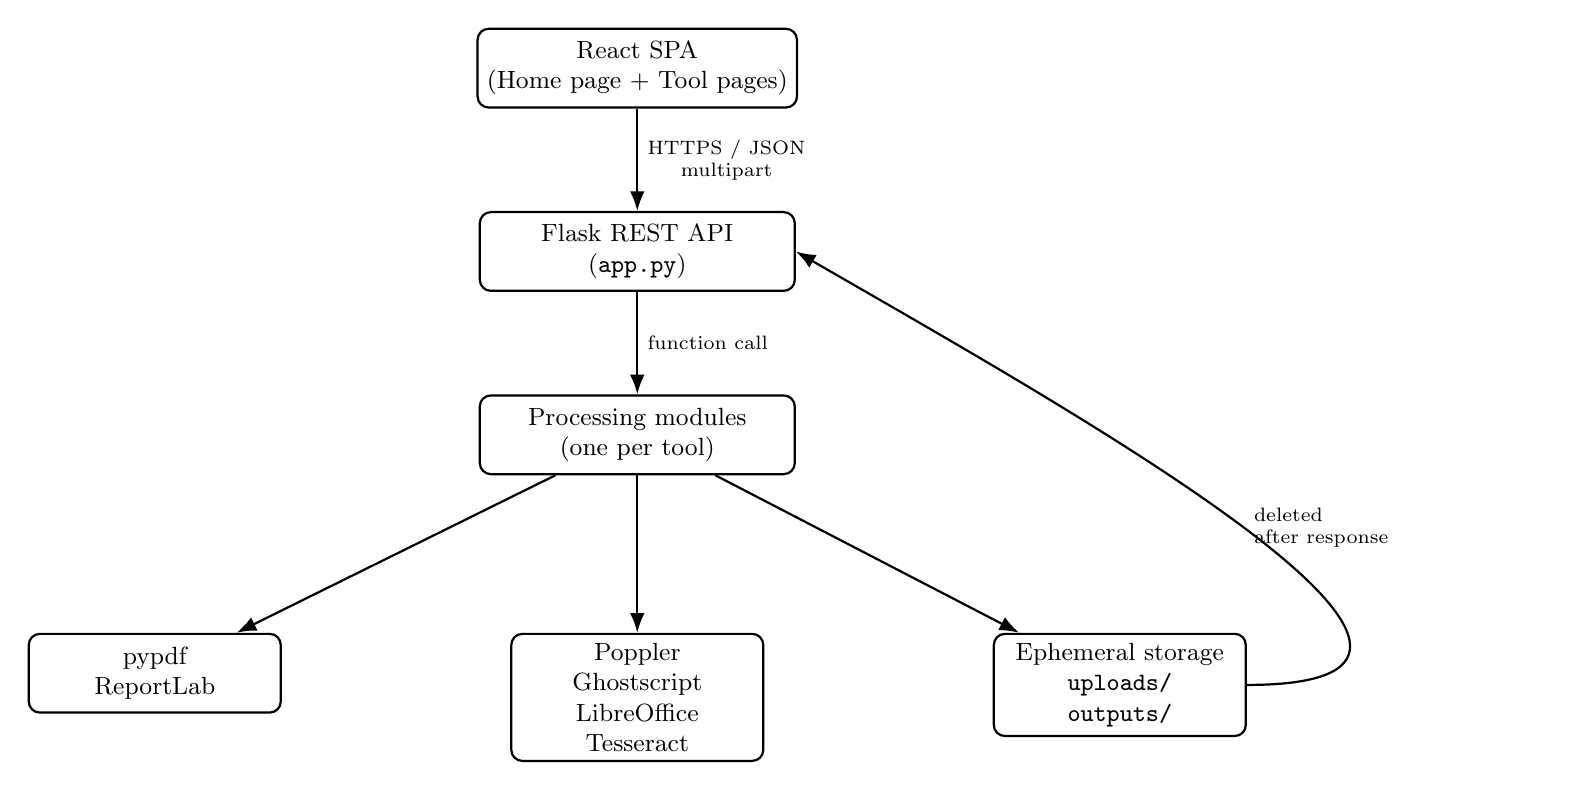
\begin{tikzpicture}[
    node distance=1.3cm,
    box/.style={
        draw,
        thick,
        rounded corners,
        minimum width=4cm,
        minimum height=1cm,
        align=center,
        font=\small
    },
    smallbox/.style={
        draw,
        thick,
        rounded corners,
        minimum width=3.2cm,
        minimum height=1cm,
        align=center,
        font=\small
    },
    arr/.style={
        -{Latex[length=2.5mm]},
        thick
    }
]

% Main vertical flow
\node[box] (client) {React SPA\\(Home page + Tool pages)};
\node[box, below=of client] (api) {Flask REST API\\(\texttt{app.py})};
\node[box, below=of api] (modules) {Processing modules\\(one per tool)};

% Bottom layer
\node[smallbox, below left=2cm and 2.5cm of modules] (pure)
{pypdf\\ReportLab};

\node[smallbox, below=2cm of modules] (bin)
{Poppler\\Ghostscript\\LibreOffice\\Tesseract};

\node[smallbox, below right=2cm and 2.5cm of modules] (fs)
{Ephemeral storage\\\texttt{uploads/}\\\texttt{outputs/}};

% Connections
\draw[arr]
(client) --
node[right, font=\scriptsize, align=center]
{HTTPS / JSON\\multipart}
(api);

\draw[arr] (api) -- node[right,font=\scriptsize]
{function call} (modules);

\draw[arr] (modules) -- (pure);
\draw[arr] (modules) -- (bin);
\draw[arr] (modules) -- (fs);

% Cleanup arrow
\draw[arr]
(fs.east)
to[out=0,in=-30,looseness=1.3]
node[right,font=\scriptsize,align=left]
{deleted\\after response}
(api.east);

\end{tikzpicture}

\caption{High-level system architecture}
\label{fig:architecture}
\end{figure}

\section{Request Life Cycle}
Every write endpoint (all endpoints except \texttt{/health}) follows the same five-step life
cycle, shown in Figure~\ref{fig:lifecycle}. This uniform pattern is what allows twelve
functional requirements to be implemented with a consistent, predictable error-handling
strategy.
\begin{figure}[h]
\centering
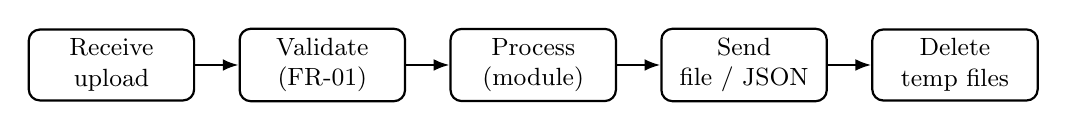
\begin{tikzpicture}[
  block/.style={
    draw,
    thick,
    rounded corners,
    minimum height=0.9cm,
    minimum width=2.1cm,
    align=center,
    font=\small
  },
  arr/.style={-{Latex[length=2mm]}, thick}
]

\node[block] (a) {Receive\\upload};
\node[block, right=0.55cm of a] (b) {Validate\\(FR-01)};
\node[block, right=0.55cm of b] (c) {Process\\(module)};
\node[block, right=0.55cm of c] (d) {Send\\file / JSON};
\node[block, right=0.55cm of d] (e) {Delete\\temp files};

\draw[arr] (a) -- (b);
\draw[arr] (b) -- (c);
\draw[arr] (c) -- (d);
\draw[arr] (d) -- (e);

\end{tikzpicture}
\caption{Request life cycle common to every endpoint}
\label{fig:lifecycle}
\end{figure}

If validation in step 2 fails, the pipeline short-circuits directly to a JSON error response and
step 5, so a rejected upload is deleted immediately rather than left on disk.

\section{User Interface Design}
The interface was deliberately designed as a multi-page application rather than a single form
with a dropdown, so that a user arriving at any tool can see, and reach, every other tool without
returning to the home page. Figure~\ref{fig:wireframe} shows the two page layouts side by side.
The home page groups the ten tools into three categories --- Organize, Convert, and Optimize ---
and the tool page keeps the same grouped list visible as a permanent sidebar, with the active
tool highlighted.

\begin{figure}[h]
\centering
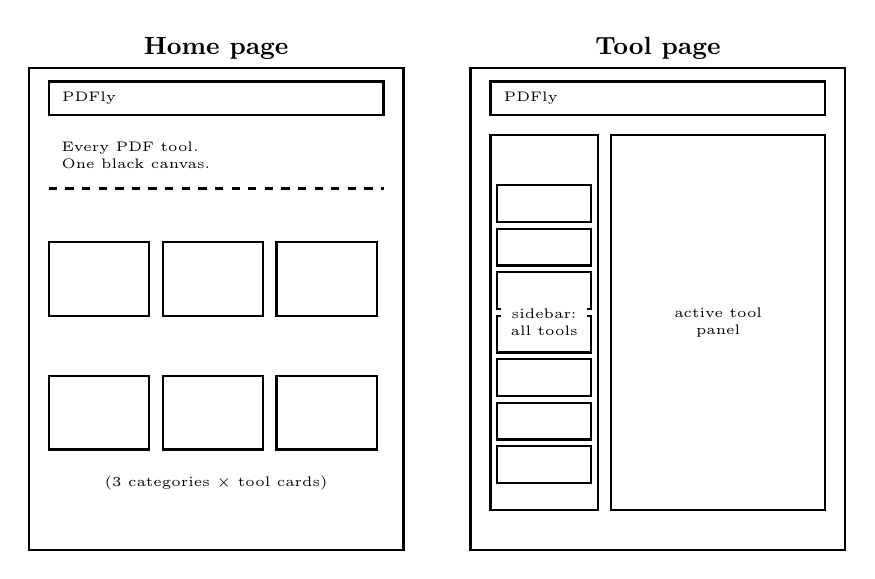
\begin{tikzpicture}[scale=0.85, every node/.style={font=\tiny}]

% ---- Home page wireframe ----
\draw[thick] (0,0) rectangle (5.6,7.2);
\node at (2.8,7.5) [font=\small\bfseries] {Home page};
\draw[thick] (0.3,6.5) rectangle (5.3,7);
\node at (0.9,6.75) {PDFly};
\draw[thick,dashed] (0.3,5.4) -- (5.3,5.4);
\node[align=left] at (1.6,5.9) {Every PDF tool.\\One black canvas.};
\foreach \r in {0,1} {
  \foreach \c in {0,1,2} {
    \draw[thick] (0.3+1.7*\c,3.5-2*\r) rectangle (1.8+1.7*\c,4.6-2*\r);
  }
}
\node at (2.8,1.0) {(3 categories $\times$ tool cards)};

% ---- Tool page wireframe ----
\begin{scope}[xshift=6.6cm]
\draw[thick] (0,0) rectangle (5.6,7.2);
\node at (2.8,7.5) [font=\small\bfseries] {Tool page};
\draw[thick] (0.3,6.5) rectangle (5.3,7);
\node at (0.9,6.75) {PDFly};
\draw[thick] (0.3,0.6) rectangle (1.9,6.2);
\foreach \y in {0,1,...,6} {
  \draw[thick] (0.4,1.0+0.65*\y) rectangle (1.8,1.55+0.65*\y);
}
\node[align=center] at (1.1,3.4) [fill=white] {sidebar:\\all tools};
\draw[thick] (2.1,0.6) rectangle (5.3,6.2);
\node[align=center] at (3.7,3.4) {active tool\\panel};
\end{scope}
\end{tikzpicture}
\caption{Wireframe of the home page (left) and the tool page (right)}
\label{fig:wireframe}
\end{figure}

A single color-coding rule runs through both layouts: every tool is assigned one accent color,
used consistently for its icon badge on the home page and for its highlighted state in the
sidebar. Outside of that one rule, the interface uses a plain black background and a single
neutral accent for primary buttons, so that color is used only to help the user locate a tool,
never as decoration.

% =========================================================================
\chapter{Implementation}
% =========================================================================

\section{Technology Stack}
\begin{table}[h]
\centering
\caption{Technology stack}
\label{tab:stack}
\begin{tabular}{@{}p{2.6cm}p{9.5cm}@{}}
\toprule
\textbf{Layer} & \textbf{Technologies} \\
\midrule
Backend language & Python 3.10+ \\
Backend framework & Flask 3.0, with Flask-CORS for cross-origin requests \\
PDF processing & pypdf, ReportLab, pdf2docx, pdfplumber, PyMuPDF, Pillow \\
External binaries & Poppler (\texttt{pdftoppm}), Ghostscript, LibreOffice (\texttt{soffice}), Tesseract OCR \\
Background jobs & APScheduler (interval-based cleanup sweep) \\
Production server & Gunicorn (WSGI) \\
Frontend framework & React 18, built with Vite \\
Frontend routing & react-router-dom (\texttt{HashRouter}) \\
Styling & Hand-written CSS with custom properties (no CSS framework) \\
\bottomrule
\end{tabular}
\end{table}

\section{Backend Implementation}

\subsection{Project Structure}
\begin{lstlisting}[language=bash, caption={Backend directory layout}, label=lst:structure]
backend/
  app.py            Flask app - route table and error handlers
  cleanup.py        Background sweep job (FR-10)
  requirements.txt
  modules/
    validators.py   Upload validation (FR-01)
    merge.py        FR-02
    split.py        FR-03
    compress.py     FR-04  (shells out to Ghostscript)
    convert.py      FR-05  (shells out to Poppler)
    toword.py       FR-06  (pdf2docx + pdfplumber + Tesseract fallback)
    watermark.py    FR-07  (ReportLab overlay)
    rotate.py       FR-08
    wordtopdf.py    FR-11  (shells out to LibreOffice)
    imagetopdf.py   FR-12
    editpdf.py       FR-13
  uploads/          temporary, auto-cleaned
  outputs/          temporary, auto-cleaned
\end{lstlisting}

\subsection{Upload Validation}
Every endpoint that accepts a file first passes it through \texttt{validators.py}, which checks
the file extension, MIME type, and size, and sanitizes the filename before it is ever written to
disk. Listing~\ref{lst:sanitize} shows the filename sanitizer, which strips path separators and
collapses any character outside a safe whitelist, closing off path-traversal attempts such as a
filename of \texttt{../../etc/passwd.pdf}.

\begin{lstlisting}[language=Python, caption={Filename sanitization in \texttt{validators.py}}, label=lst:sanitize]
def sanitize_filename(filename):
    """Strips path separators and any character outside a safe whitelist."""
    filename = os.path.basename(filename or "")
    filename = filename.replace("..", "")
    filename = re.sub(r'[^A-Za-z0-9._-]', "_", filename)
    if not filename:
        filename = "file.pdf"
    return filename
\end{lstlisting}

\subsection{The Compress Module}
The Compress tool (FR-04) is a thin wrapper around Ghostscript's \texttt{pdfwrite} device. It
also implements a small safety check: if the recompressed file turns out to be larger than the
original (which can happen with PDFs that are already well optimized), the original file is
returned unchanged and a notice header is attached to the response instead of silently returning
a larger file.

\begin{lstlisting}[language=Python, caption={Fallback logic in \texttt{compress.py}}, label=lst:compress]
original_size = os.path.getsize(input_path)
compressed_size = os.path.getsize(output_path)

note = None
if compressed_size >= original_size:
    os.remove(output_path)
    shutil.copyfile(input_path, output_path)
    compressed_size = original_size
    note = "Compression did not reduce file size; original file returned."
\end{lstlisting}

\subsection{Ephemeral Storage and Cleanup}
No file is meant to live on the server for longer than the request that created it. Every route
registers an \texttt{after\_this\_request} hook that deletes the uploaded and generated files as
soon as the response has been sent (Listing~\ref{lst:route}). This is not sufficient on its own,
because a client that disconnects mid-download would leave the hook without a completed response
to attach to; the background sweep in \texttt{cleanup.py} is the safety net for exactly that
case, deleting anything older than thirty seconds on a fixed interval, independent of any single
request.

\begin{lstlisting}[language=Python, caption={Per-request cleanup hook, from \texttt{app.py}}, label=lst:route]
@app.route("/merge", methods=["POST"])
def merge_route():
    files = request.files.getlist("files")
    ...
    output_path = new_output_path("merged")
    merge_pdfs(saved_paths, output_path)

    @after_this_request
    def _cleanup(response):
        cleanup_paths(*saved_paths, output_path)
        return response

    return send_file(output_path, as_attachment=True,
                      download_name="merged_output.pdf")
\end{lstlisting}

\subsection{Error Handling}
All twelve processing endpoints follow the same \texttt{try/except} shape: a
\texttt{ValidationError} raised anywhere in the pipeline is caught and turned into a JSON error
object with the appropriate HTTP status code, and any other exception is logged server-side and
turned into a generic 400 or 500 response, so that an unexpected failure in a third-party library
never leaks an internal stack trace to the client.

\section{Frontend Implementation}

\subsection{Single Source of Truth for Tool Metadata}
Every tool's label, description, icon, category, accent color, and React component are declared
once, in \texttt{toolsConfig.js}. Both the home page grid and the tool page sidebar read from
this same array, so adding an eleventh tool in the future requires one new entry in one file
rather than edits scattered across several components.

\begin{lstlisting}[language=Javascript, caption={One entry from \texttt{toolsConfig.js}}, label=lst:toolsconfig]
{
  key: "compress",
  label: "Compress PDF",
  short: "Shrink file size",
  description: "Reduce a PDF's file size while keeping it readable.",
  icon: "compress",
  color: "#3FCB86",
  category: "Optimize",
  component: CompressPanel,
}
\end{lstlisting}

\subsection{Routing}
The application uses \texttt{react-router-dom} with two routes: \texttt{/} for the home page and
\texttt{/tool/:toolKey} for every tool page. \texttt{HashRouter} was chosen deliberately over
\texttt{BrowserRouter} so that the production build works from any static file server without
server-side rewrite rules having to be configured separately.

\subsection{Consistent API Error Handling}
All ten tool panels call through a single \texttt{api.js} module rather than calling
\texttt{fetch} directly. This module distinguishes a network failure from an HTTP error returned
by the server and always surfaces the backend's own error message where one is available, so
every panel shows the same style of error regardless of which endpoint failed.

% =========================================================================
\chapter{Testing}
% =========================================================================

\section{Testing Strategy}
Because the system has no persistent state, testing focused on running each endpoint against a
live server with real generated PDFs, rather than only unit-testing individual functions in
isolation. Each functional requirement was exercised at least once against its success path and
at least once against its documented failure path.

\section{Test Cases and Results}
\begin{longtable}{@{}p{9cm}p{2.2cm}@{}}
\toprule
\textbf{Test case} & \textbf{Result} \\
\midrule
\endhead
Merge two or more files $\rightarrow$ correct combined page count & Passed \\
Merge with only one file $\rightarrow$ HTTP 400 & Passed \\
Split a valid page range $\rightarrow$ correct pages extracted & Passed \\
Split an out-of-range page $\rightarrow$ HTTP 400 with page count in message & Passed \\
Rotate 90/180/270 $\rightarrow$ \texttt{/Rotate} property set correctly & Passed \\
Rotate an invalid angle (45) $\rightarrow$ HTTP 400 & Passed \\
Watermark with valid text $\rightarrow$ applied to every page & Passed \\
Watermark with empty text $\rightarrow$ HTTP 400 & Passed \\
Convert a multi-page PDF $\rightarrow$ ZIP of PNGs & Passed \\
Convert a single-page PDF $\rightarrow$ single PNG & Passed \\
Compress $\rightarrow$ original/compressed sizes reported in headers & Passed \\
Compress a file that cannot shrink further $\rightarrow$ original returned with notice & Passed \\
PDF to Word $\rightarrow$ valid, openable .docx & Passed \\
Wrong file type upload $\rightarrow$ HTTP 400 & Passed \\
Zero-byte file upload $\rightarrow$ HTTP 400 & Passed \\
Path-traversal filename (\texttt{../../etc/passwd.pdf}) $\rightarrow$ sanitized & Passed \\
Five concurrent requests $\rightarrow$ all succeed, no cross-contamination & Passed \\
Files removed from \texttt{uploads/}/\texttt{outputs/} after every request & Passed \\
CORS preflight from the frontend origin & Passed \\
Backend imports cleanly with all dependencies installed & Passed \\
Frontend production build (\texttt{npm run build}) & Passed, no errors \\
\bottomrule
\caption{Functional test cases and outcomes}
\label{tab:tests}
\end{longtable}

\section{Defects Found During Verification}
Two defects were found and corrected during a later end-to-end verification pass, both worth
recording because they illustrate the difference between ``the build succeeds'' and ``the server
actually starts and answers requests'', which this project treated as two separate checks.

\begin{enumerate}[label=\arabic*.]
  \item \textbf{Empty module file contained placeholder text.} \texttt{modules/\_\_init\_\_.py}
        contained the literal text \texttt{(empty)} rather than being an empty file, which is
        valid Python only inside a string but raised \texttt{NameError: name 'empty' is not
        defined} when the module was imported as bare code. The fix was to make the file
        genuinely empty.
  \item \textbf{Missing dependencies in \texttt{requirements.txt}.} The PDF-to-Word module
        imports \texttt{PyMuPDF}, \texttt{Pillow}, \texttt{pdf2docx}, \texttt{pdfplumber}, and
        \texttt{pytesseract} at the top of the file, none of which were listed in
        \texttt{requirements.txt}. A fresh install therefore failed on \texttt{import app} before
        the Flask server ever started. All five packages were added and pinned, and the fix was
        verified by installing into a clean virtual environment, importing the app directly,
        starting the real development server, and confirming that \texttt{GET /health} returned
        \texttt{200} and a deliberately invalid \texttt{POST /merge} returned \texttt{400}.
\end{enumerate}

% =========================================================================
\chapter{Result and Discussion}
% =========================================================================

\section{Outcome}
The resulting system exposes twelve functional requirements through twelve HTTP endpoints, all of
which were exercised against a running server rather than validated only by a successful code
compile. The frontend presents these as ten user-facing tools, grouped into three categories, with
a consistent visual language --- one accent color per tool, reused on both the home page and the
in-tool sidebar --- as the only place color is used for anything other than plain text and
buttons.

\section{Discussion}
The decision to delegate almost all PDF-processing logic to established libraries and
command-line tools, rather than implementing parsing or rendering from scratch, kept the
project's own code small (approximately 1,400 lines of backend Python and a comparable amount of
frontend JavaScript) while still covering twelve distinct requirements. The trade-off is a
dependency on external binaries --- Poppler, Ghostscript, LibreOffice, and Tesseract --- which
must be separately installed on whichever machine runs the backend, a cost that was made explicit
in the project's setup documentation rather than discovered by a user at run time.

The two defects described in Chapter 5 also highlight a limitation of relying on
\texttt{npm run build} or a static code read as evidence that a project ``works'': neither would
have caught a backend that fails on \texttt{import}, because the build step never touches the
backend at all. Actually starting the server and sending it a request was what surfaced both
issues.

% =========================================================================
\chapter{Conclusion and Future Work}
% =========================================================================

\section{Conclusion}
This project set out to build a self-hosted alternative to commercial web-based PDF tools,
covering merge, split, rotate, watermark, compression, page-level editing, and four conversion
operations, without requiring user accounts or persistent storage of uploaded documents. All
twelve functional requirements were implemented, and each was verified against its success path
and at least one failure path on a running server. The frontend was designed so that every tool
remains one click away from every other tool, addressing the specific usability goal set out in
Chapter 1.

\section{Limitations}
\begin{itemize}
  \item The system has no persistent storage or user accounts; a processed file must be
        downloaded immediately, as nothing is kept for a later session.
  \item Several tools depend on external binaries (Poppler, Ghostscript, LibreOffice, Tesseract)
        that must be installed separately from the Python dependencies, which adds friction to
        deployment, particularly on Windows.
  \item Processing is synchronous and single-threaded per request; a very large file could block
        the request for the duration of its processing time.
  \item The OCR fallback in the PDF-to-Word tool only handles scanned pages with no existing text
        layer; it is not a full OCR-based document reconstruction pipeline.
\end{itemize}

\section{Future Work}
\begin{itemize}
  \item Add optional user accounts with a personal, time-limited file history, backed by a
        lightweight database.
  \item Move long-running conversions (large PDF-to-Word jobs, batch image conversion) to an
        asynchronous task queue so the HTTP request does not block on processing.
  \item Add drag-to-reorder for the Merge and Image-to-PDF tools instead of relying on upload
        order.
  \item Package the external binary dependencies into a single Docker image to remove the
        separate installation step from the deployment process.
  \item Add a lightweight test suite (e.g. \texttt{pytest}) that runs the same test cases listed
        in Table~\ref{tab:tests} automatically in a continuous-integration pipeline.
\end{itemize}

% =========================================================================
\begin{thebibliography}{99}
\addcontentsline{toc}{chapter}{References}

\bibitem{flask} Flask Documentation. \textit{Flask: A Python Micro Web Framework.}
  \url{https://flask.palletsprojects.com/}

\bibitem{react} React Documentation. \textit{React -- A JavaScript Library for Building User
  Interfaces.} \url{https://react.dev/}

\bibitem{pypdf} pypdf Documentation. \textit{pypdf: A Pure-Python PDF Library.}
  \url{https://pypdf.readthedocs.io/}

\bibitem{reportlab} ReportLab Documentation. \textit{ReportLab PDF Toolkit for Python.}
  \url{https://www.reportlab.com/docs/reportlab-userguide.pdf}

\bibitem{poppler} Poppler Project. \textit{Poppler: A PDF Rendering Library.}
  \url{https://poppler.freedesktop.org/}

\bibitem{ghostscript} Artifex Software. \textit{Ghostscript Documentation.}
  \url{https://www.ghostscript.com/docs/}

\bibitem{libreoffice} The Document Foundation. \textit{LibreOffice Headless Command-Line
  Conversion.} \url{https://help.libreoffice.org/}

\bibitem{tesseract} Google / Tesseract OCR. \textit{Tesseract Open Source OCR Engine.}
  \url{https://github.com/tesseract-ocr/tesseract}

\bibitem{ilovepdf} iLovePDF. \textit{Online PDF Tools for PDF Lovers.}
  \url{https://www.ilovepdf.com/}

\bibitem{vite} Vite Documentation. \textit{Vite: Next Generation Frontend Tooling.}
  \url{https://vitejs.dev/}

\end{thebibliography}

% =========================================================================
\appendix
\chapter{REST API Reference}
\addcontentsline{toc}{chapter}{Appendix A: REST API Reference}

\begin{longtable}{@{}p{1.6cm}p{2.6cm}p{4.2cm}p{4.5cm}@{}}
\toprule
\textbf{Method} & \textbf{Endpoint} & \textbf{Request} & \textbf{Response} \\
\midrule
\endhead
POST & \texttt{/merge} & \texttt{files[]} (2+ PDFs) & merged PDF \\
POST & \texttt{/split} & \texttt{file}, \texttt{range} & PDF of extracted pages \\
POST & \texttt{/rotate} & \texttt{file}, \texttt{angle} & rotated PDF \\
POST & \texttt{/watermark} & \texttt{file}, \texttt{text} & watermarked PDF \\
POST & \texttt{/convert} & \texttt{file}, \texttt{format} & image or ZIP of images \\
POST & \texttt{/imagetopdf} & \texttt{files[]} (1+ images) & PDF \\
POST & \texttt{/compress} & \texttt{file} & compressed PDF, with size headers \\
POST & \texttt{/toword} & \texttt{file} & \texttt{.docx} \\
POST & \texttt{/wordtopdf} & \texttt{file} (.docx) & PDF \\
POST & \texttt{/edit/inspect} & \texttt{file} & JSON page structure \\
POST & \texttt{/edit/apply} & \texttt{file}, \texttt{edits} (JSON) & edited PDF \\
GET & \texttt{/health} & --- & \texttt{\{"status": "ok"\}} \\
\bottomrule
\caption{Complete REST API endpoint reference}
\label{tab:api}
\end{longtable}

\chapter{Sample Error Response}
\addcontentsline{toc}{chapter}{Appendix B: Sample Error Response}
Every error response returned by the backend follows the same JSON shape, regardless of which
endpoint or which validation rule triggered it:

\begin{lstlisting}[language=Python, caption={Uniform error response shape}]
{
  "error": true,
  "message": "Only PDF files are accepted."
}
\end{lstlisting}

\end{document}
